\documentclass[letterpaper, 11pt]{article}
\usepackage[utf8]{inputenc}
\usepackage{graphicx}
\usepackage[style=numeric, citestyle=authoryear]{biblatex}
%\bibliographystyle{apalike}
\usepackage{rotating}
\addbibresource{mendeley.bib}
\usepackage{indentfirst}
\usepackage[margin = 0.5 in]{geometry}
\usepackage{xcolor}
\usepackage{setspace}
\usepackage{wrapfig}



\title{Chapter 1: The effects of floodplain shade on hyporheic zone temperatures}
\author{Katie Fogg}
\date{}

\begin{document}

\maketitle

\section{Introduction}
\begin{itemize}
    \item Hyporheic exchange regulates stream channel temperatures in floodplain stream reaches \parencite{Arrigoni2008BufferedChannels}. In floodplain streams flowing over expansive, coarse-grained alluvial aquifers, the effects of hyporheic exchange on the in-stream environment are especially pronounced.
    
    \item Floodplain hyporheic zones are typically wide and shallow. In the famously large Nyack floodplain of the middle fork of the Flathead River, the alluvial aquifer spans up to 1.5 kilometers wide, which saturated depths between 6 and 25 meters with 1 to 3 meters of fine sediments on the floodplain overlying the aquifer \parencite{Helton2014RelativeFloodplain}. 

    \item Because of the broad and shallow nature of floodplains, we hypothesize that landscape features on the floodplain surface, specifically the presence or absence of trees and their associated shade, affect the temperature of the hyporheic zone by reducing solar radiation on the ground surface, thereby reducing the conduction of heat through the floodplain sediments overlying the hyporheic zone. 
    
    \item Excessive heating of the hyporheic zone via increased solar radiation has been speculated in the past but not directly studied. Blah Blah studied stream temperature before and after clear-cut forest harvesting and found that after tree harvest, the stream  temperature warmed even though there was an intact riparian buffer strip. 
    
    \item In this paper, we conducted a simple modeling experiment to determine the effects of floodplain landscape variables on hyporheic zone temperatures. We modeled a representative hyporheic zone where we varied the thickness of the unsaturated floodplain sediments overlying the hyporheic zone, the hydraulic conductivity of the saturated porous media and altered the soil temperature boundary conditions to reflect either soil temperatures under tree shade or soil temperatures in full sun. 

\end{itemize}

%\subsection{From Proposal}
%Streams with summertime temperatures that are too hot to support native biota are a widespread management concern, particularly in the salmon-rearing streams of the Northwestern U.S. \parencite{Richter2005MaximumNorthwest}. Management practices to reduce summertime stream temperatures include increasing stream-bank vegetative shade and increasing the amount of hyporheic exchange. Increasing vegetative shade is a well-established and common practice for reducing summertime temperatures, whereas altering hyporheic exchange is a relatively new restoration practice and is much less common. 

%Increasing hyporheic exchange is most practicable in streams where hyporheic exchange is already or has a history of being a major process- such as floodplain reaches. Coincidentally, floodplain streams are most likely to be regulated via dredging, levees, etc, thus reducing hyporheic exchange. Similarly, increasing stream-side vegetation to increase shade is most befitting to streams with a history of vegetated banks.

%Both shade and hyporheic exchange have been shown to reduce the diel mean and amplitude of summertime stream channel temperatures. However, there have been some investigations where shade and hyporheic exchange did not lead to cooler temperatures.   

%\begin{wrapfigure}{R}{0.4\textwidth}
%\centering
%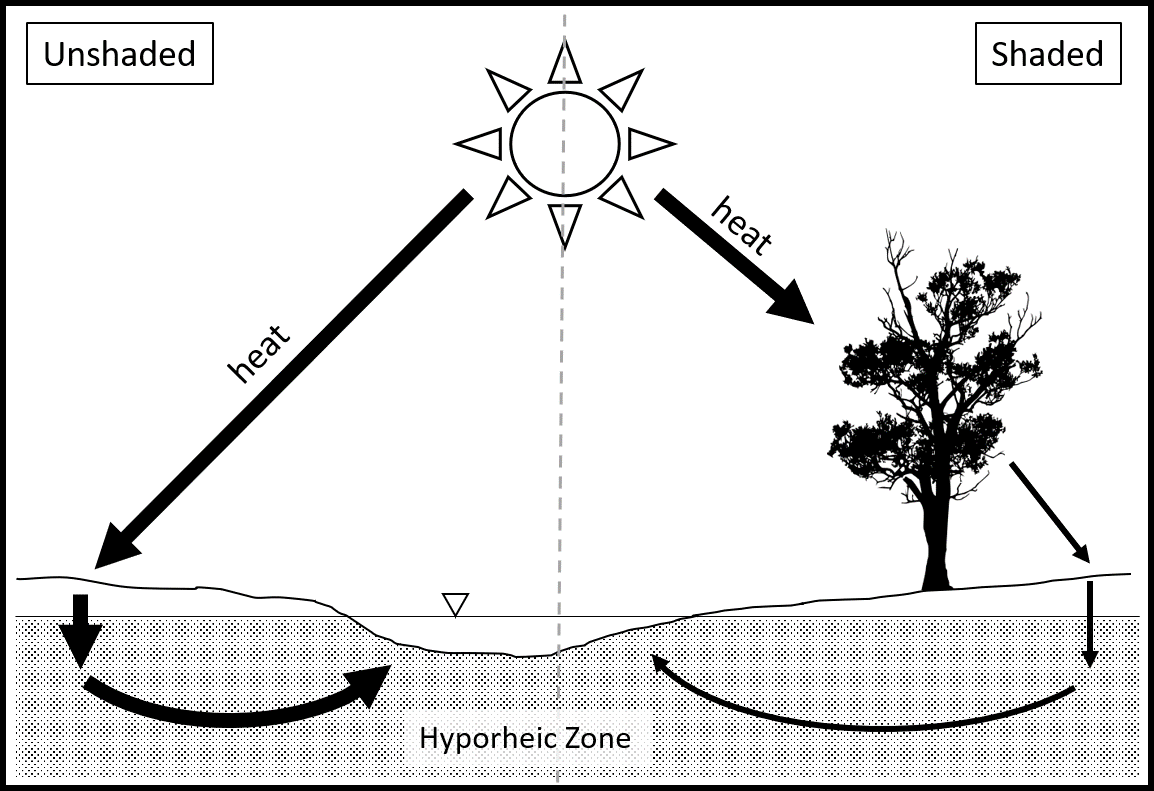
\includegraphics[width=0.4\textwidth]{Figures/ShadedAndUnshadedConceptModel.png}
%\caption{\label{fig:One} Conceptual model of how shaded and unshaded floodplains alter hyporheic and stream heat dynamics.}
%\end{wrapfigure}

%In expansive floodplains, hyporheic zones exchange substantial amounts of water with the stream channel \parencite{Stanford1993AnCorridor, Faulkner2012HyporheicAttributes}, influencing channel water temperature \parencite{Arrigoni2008BufferedChannels, Evans1998}. If floodplain vegetation alters hyporheic water temperatures, rates of hyporheic heat exchange and associated channel water temperatures will be affected. I ask ``How do various heat transfer mechanisms link floodplain shade, hyporheic temperatures, and associated channel water temperatures?''  Specifically, I hypothesize that \textbf{(1) floodplain shade influences hyporheic temperatures by reducing solar radiation on the ground surface, thereby reducing the conduction of heat through the floodplain sediments overlying the hyporheic zone}, and \textbf{(2) the spatial juxtaposition of shade and hyporheic flow paths on the floodplain govern the exchange of heat between the atmosphere, hyporheic zone, and channel, ultimately determining the magnitude of channel temperature response}. 

\section{Methods}
To understand the effects of shade on hyporheic zone temperatures, we compared hyporheic temperature from models of hyporheic zones flowing beneath either shaded or unshaded floodplain sediments. We also performed a sensitivity analysis to understand the additional temperature effects of the thickness of the overlying floodplain sediments and the values of hydraulic conductivity in the hyporheic zone. The hyporheic zone models were built in HydroGeoSphere (HGS) \cite{Aquanity2015HGSManual} which simulates terrestrial water and temperature movement. 

Our representative hyporheic zone model was a two-dimensional box with unsaturated sediment layer above it and a bedrock layer below it (Figure \ref{fig:modelgeomgrid}). The z-dimension described depth into the ground while the x-dimension described flow path length. Across all model runs, the hyporheic zone was 3 meters thick. The thickness of overlying unsaturated floodplain sediments was altered by increasing or decreasing the number of model nodes above the hyporheic zone layer. The modeled system had a 1\% slope, a value typical of a low-gradient floodplain (CITE). 
%We used a 0.1 m grid resolution in areas where the temperature variation across space was expected to be greatest.

\begin{figure}[!h]
\centering
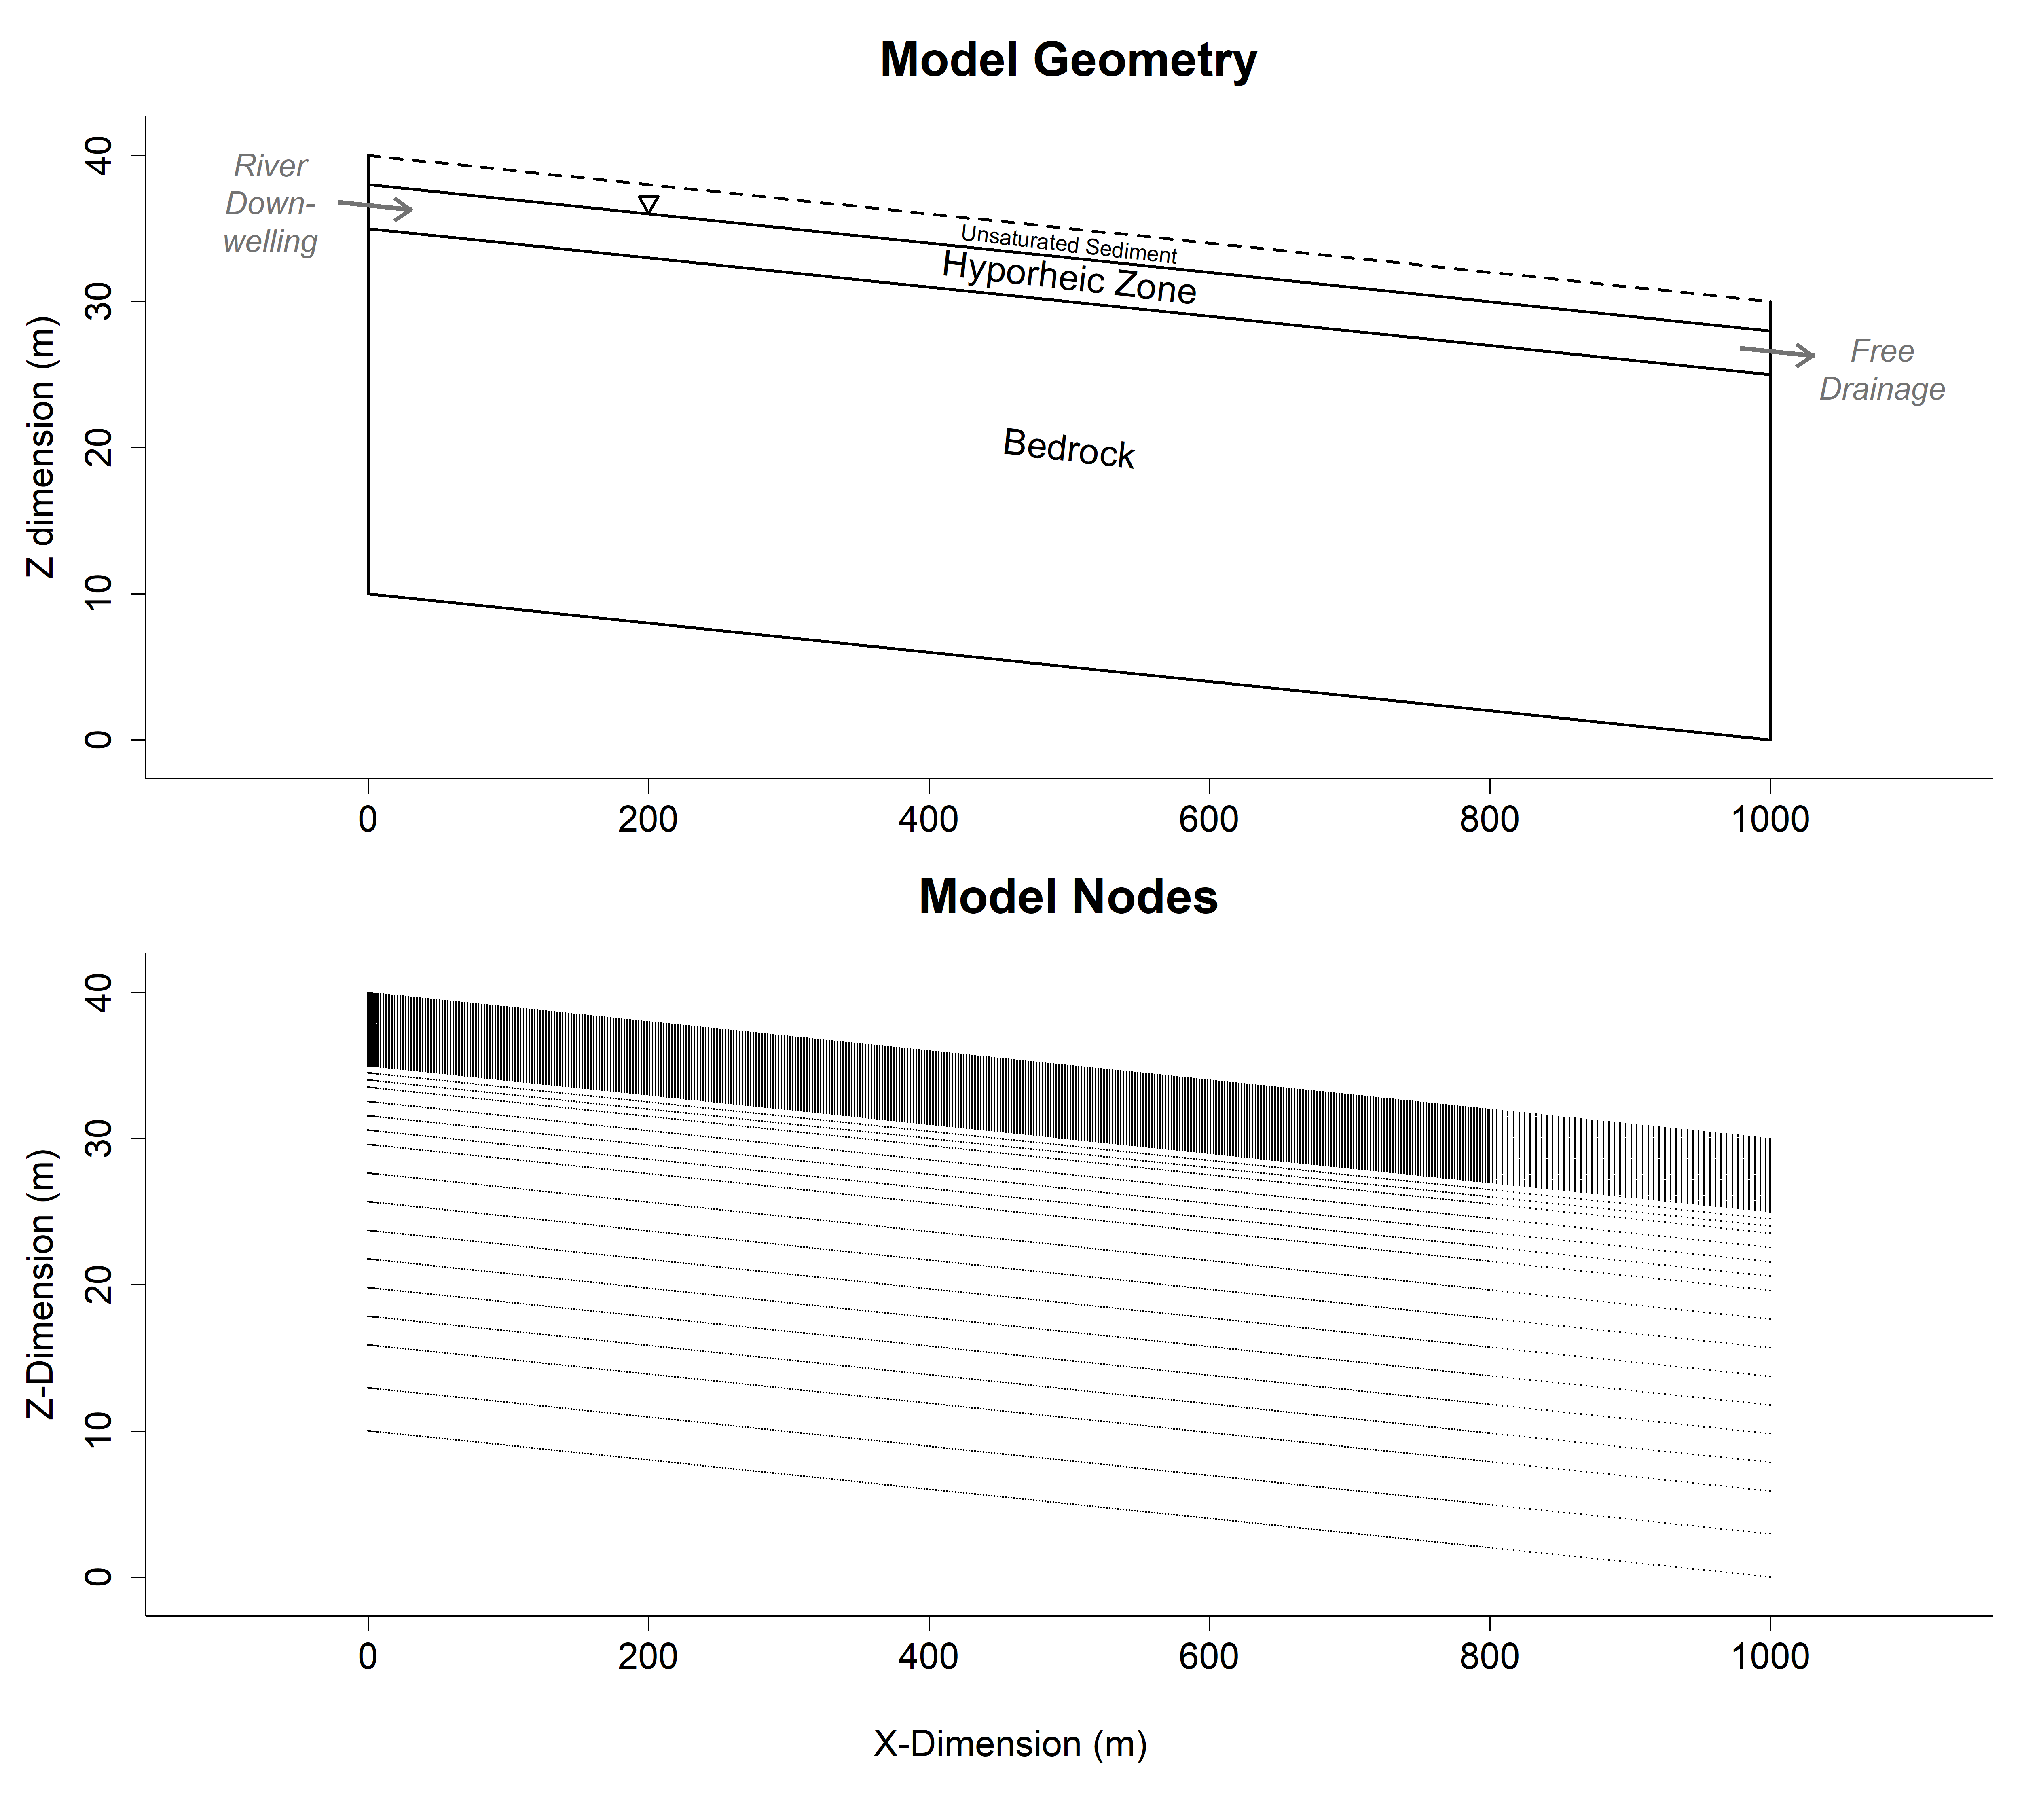
\includegraphics[width = \textwidth]{Figures/ModelGeomAndGrid.png}
\caption{Model Geometry and Nodes}
\label{fig:modelgeomgrid}
\end{figure}

We used an irregular model grid (Figure \ref{fig:modelgeomgrid}); nodes were spaced in close proximity in areas of the model domain where we expected temperature variation to be the greatest, and conversely, nodes were spaced further apart in area where we expected minimal temperature variation between nodes. In the first 4 meters in the x-dimension, a 0.1 m spacing between model nodes was used. From x = 4 m to x = 8.9 m, the node spacing linearly increased by a factor of 1.5 from 0.1 m to 2.0 m. 2.0 meter node spacing was maintained until x = 800 m. After x = 800 m, the node spacing increased to 4.0 m. In the z-direction, the node spacing was 0.1 m in the hyporheic zone and the unsaturated floodplain sediments. We increased bedrock node spacing in the z-direction, away from the bedrock-hyporheic zone boundary.






The hydrologic and thermal properties of the model were reflective of an expansive, coarse-grained basaltic alluvial aquifer overlying a nearly-impermeable bedrock layer, see Table \ref{table:hydrologyparams} and Table \ref{table:thermalparams} for hydrologic and thermal parameters. Van Genuchten equations were used to simulate unsaturated conditions above the hyporheic zone.


In our model, water entered the simulated hyporheic zone at x = 0 meters, flowed down-slope through the hyporheic zone, and drained out of the model at x = 1000 meters. We used constant head boundary conditions at both up-slope and down-slope boundaries, thus water flow into and out of the hyporheic zone did not vary across model time. The water entering the model domain was set to stream channel temperature, thus representing water downwelling from a stream channel into a hyporheic zone. For the stream channel temperatures, we used an annually repeating compound sine wave which was fit using nonlinear least squares to temperature collected from the Umatilla River, located near Pendleton, Oregon, USA (Figure \ref{fig:IskulpaaInputTemps}). The section of the Umatilla River where temperature was taken is a representative floodplain reach.

Shady and sunny floodplains conditions were represented by altering the boundary temperature at the top of the unsaturated sediment layer. A weather station located in a sunny field adjacent to the Umatilla River floodplain measured soil temperatures at 30-cm depth. Using nonlinear least squares, we fit a compound sine wave to this soil temperature data, which represented the soil boundary temperature of our 'sunny' floodplain model scenarios. The 'shady' floodplain scenario was created by altering the annual maximum and reducing the daily temperature range of the 'sunny' soil temperature (Figure \ref{fig:IskulpaaInputTemps}). These specific alterations were based off of studies by \cite{Childs1987EffectEnvironments} and \cite{Pierson1991VariabilityRangeland}, who compared shaded and unshaded soil temperatures in shelterwood and sagebrush sites.

In addition to altering floodplain shade, we varied the thickness of the overlying unsaturated floodplain sediments to further understand the interaction between the hyporheic zone and the floodplain landscape. The values of floodplain thickness that we modeled were 0.5 m, 1.0m, 2.0m and 3.0m-- encompassing a range of unsaturated sediment thickness measured in expansive alluvial floodplains at base-flow \parencite{Helton2012ScalingSystem, Munz2017CoupledDynamics}. We also varied hydraulic conductivity between 100 m day$^{-1}$ through 400 m day$^{-1}$ at 100 m day$^{-1}$ increments.

To initialize model runs we set the entire model domain to 10.3 C, the annual average river temperature. We ran each model until it reached thermal equilibrium between years (temperature difference \textless 0.1 C on January 1), and recorded the output of the final model year (year 7 for all model runs). We recorded 24 hours of modeled temperature every 15 days for one model year. We then determined the daily mean temperature for these 48 days  of output.  




%\begin{wrapfigure}{L}{0.5\textwidth}
%\begin{figure}
%\centering
%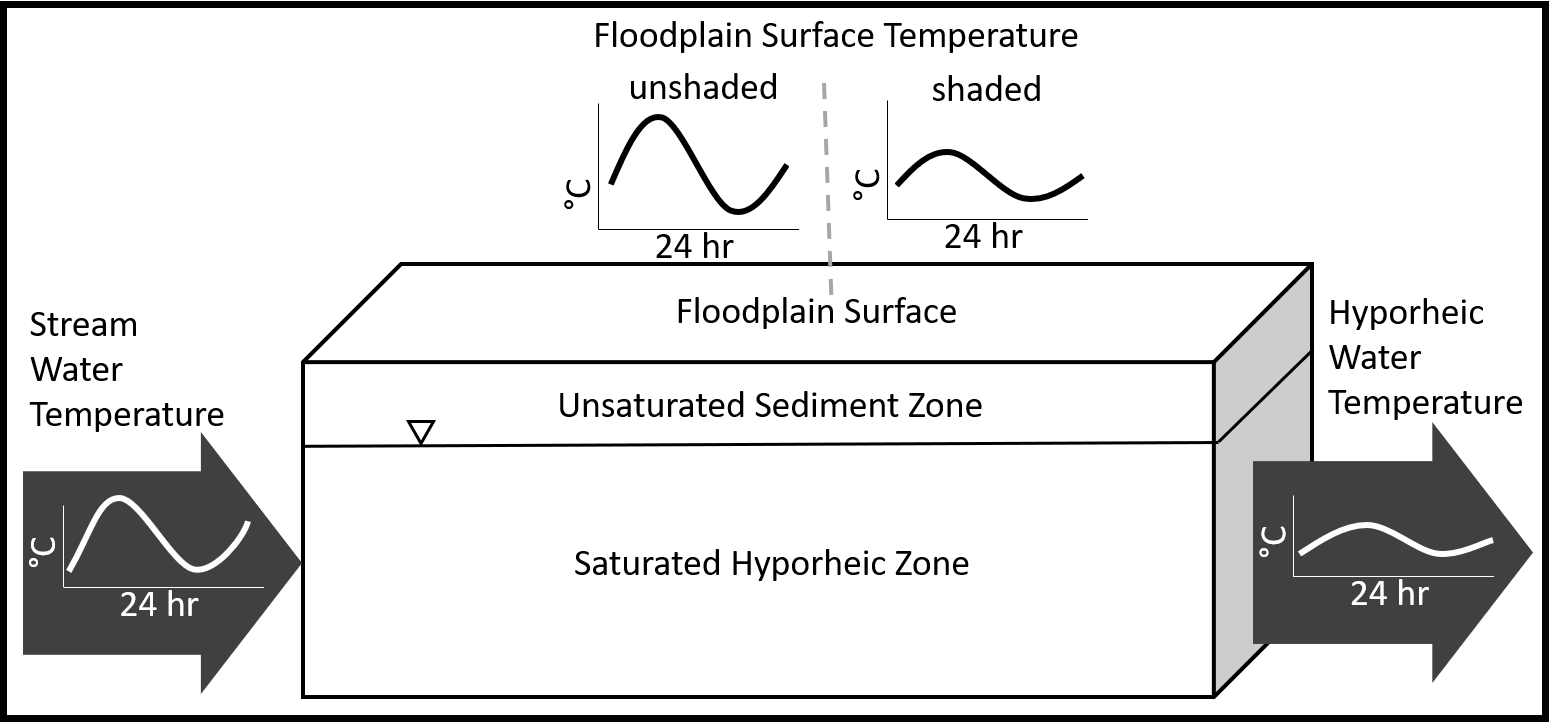
\includegraphics[width=0.5\textwidth]{ModelConceptualModel.png}
%\caption{\label{fig:Two} Diagram of hypothesis 1 HGS model. Floodplain surface has temperature of either an unshaded or shaded gravels. Stream temperature is input and hyporheic temperature is output.}
%\end{wrapfigure}
%\end{figure}

%\begin{figure}
%    \centering
%    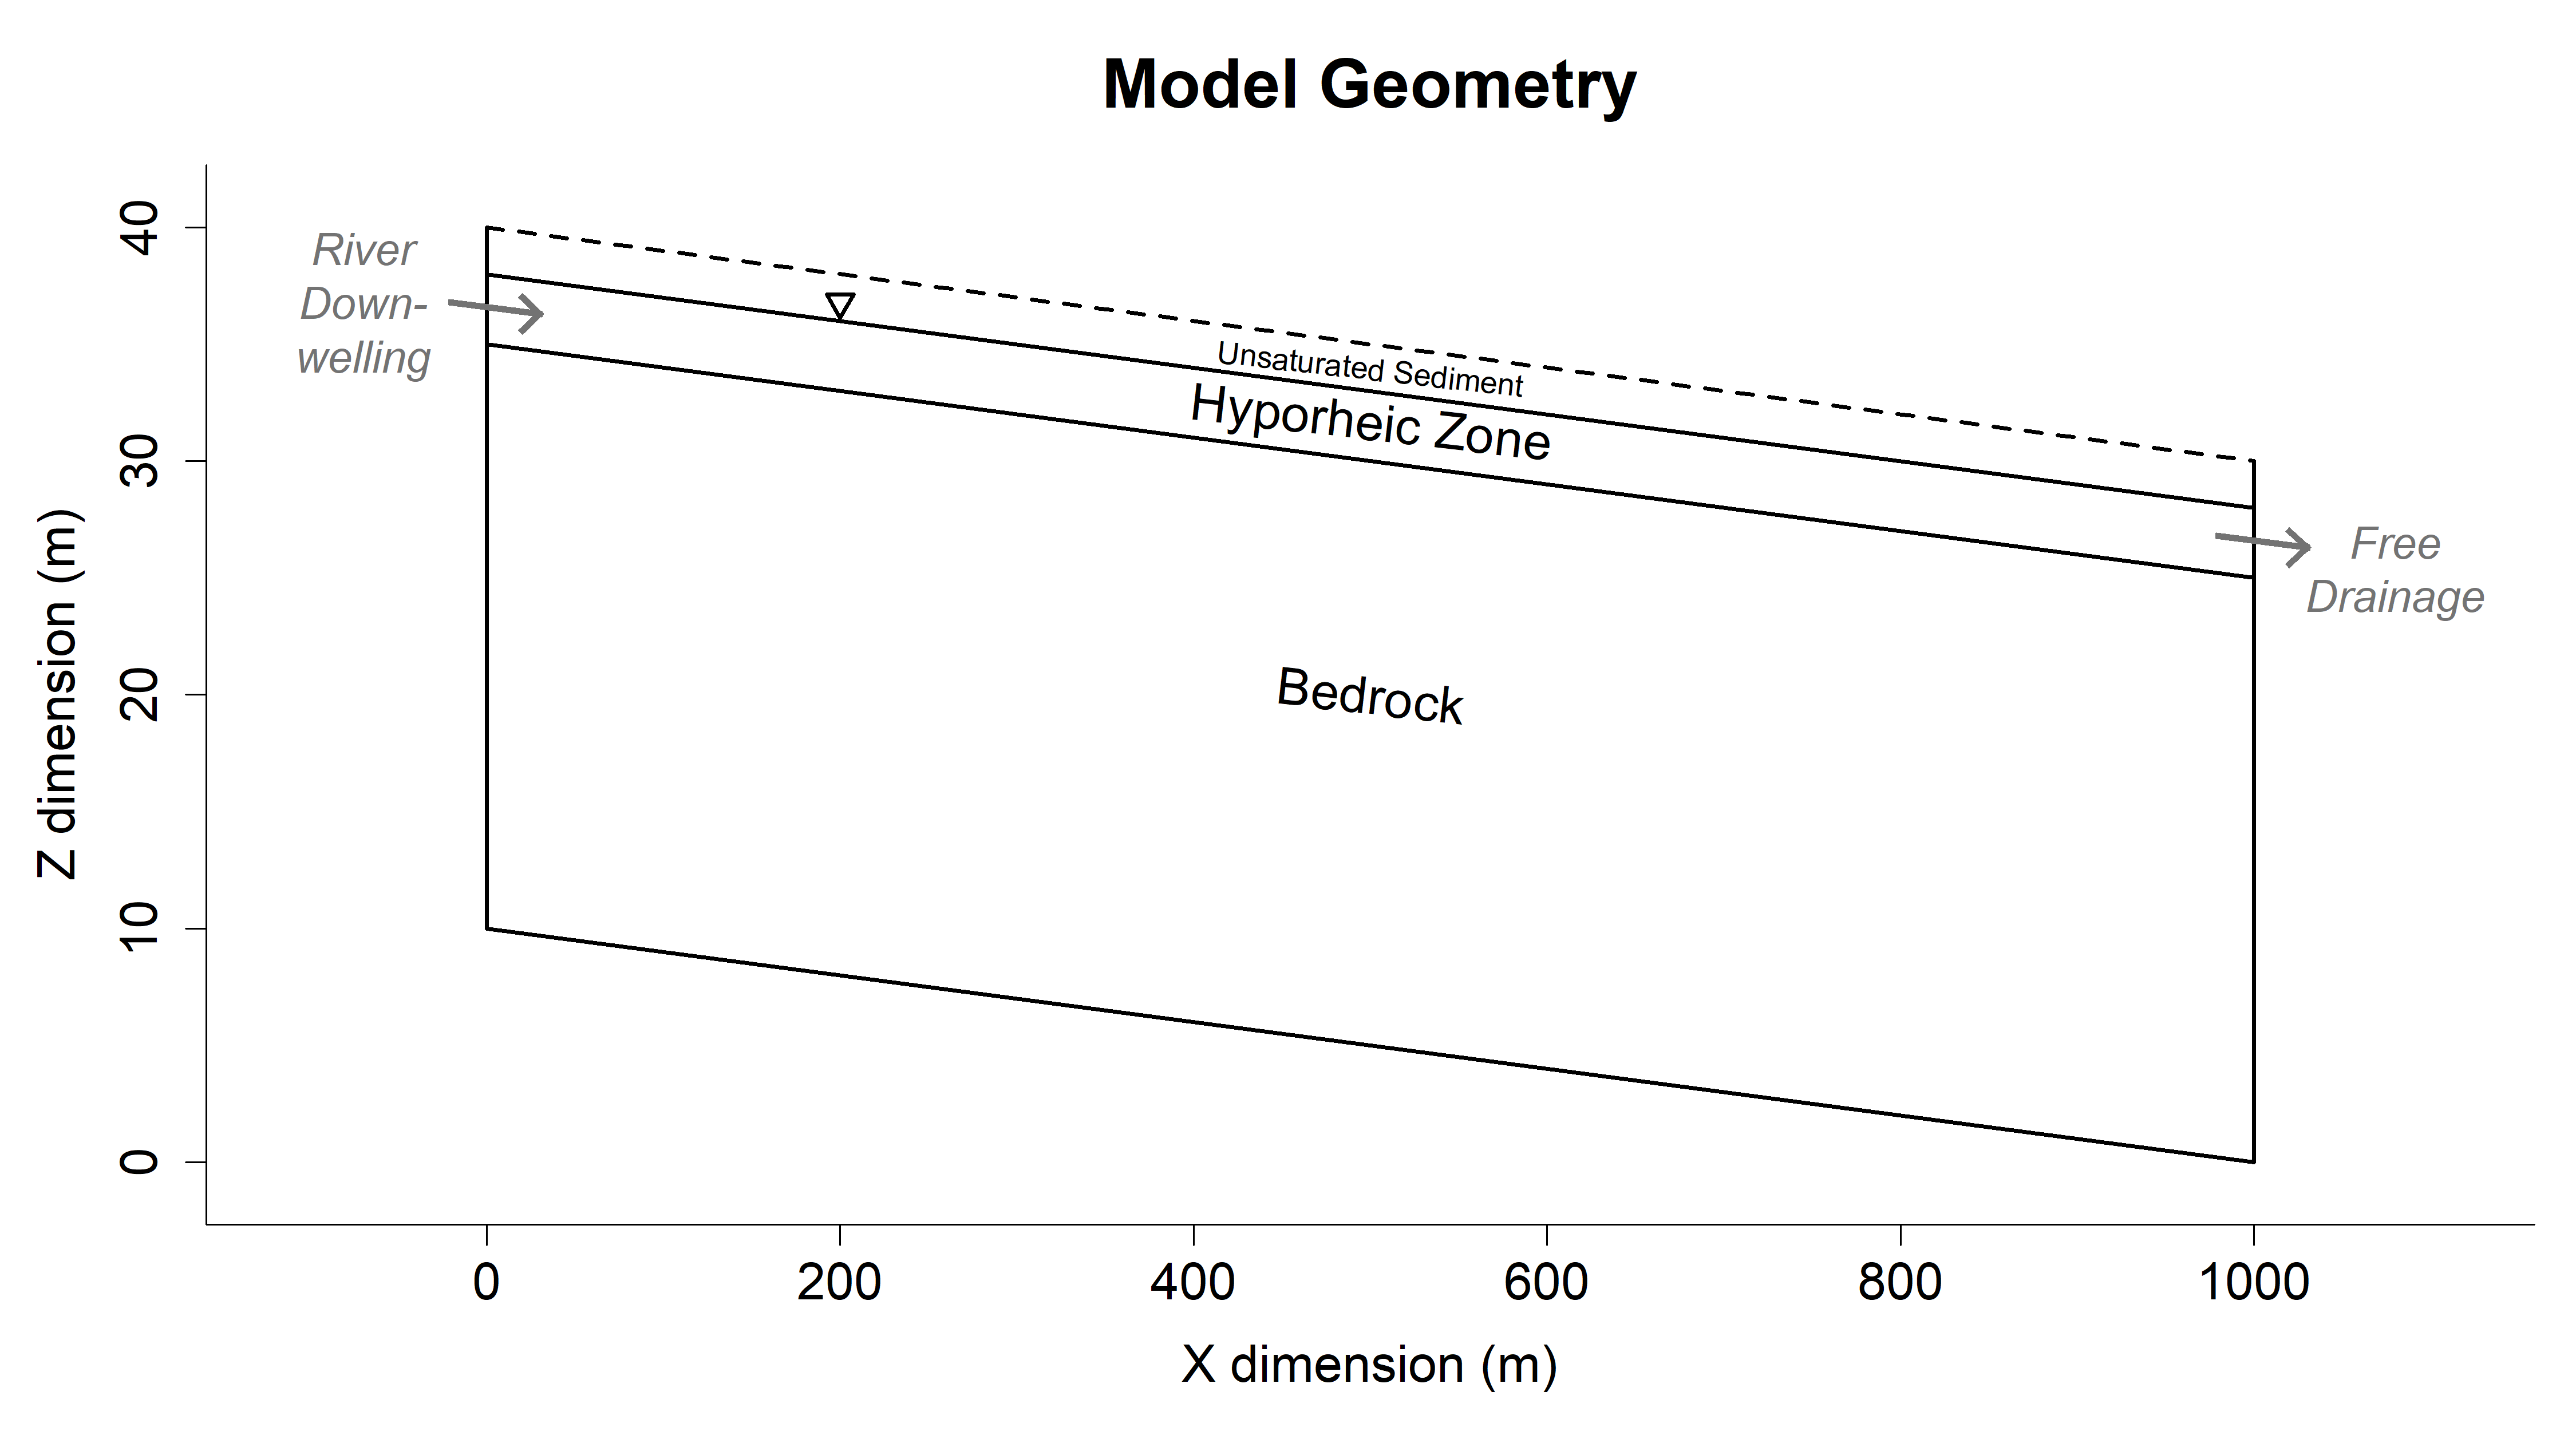
\includegraphics[width=0.8\textwidth]{ModelGeom.png}
%    \caption{ Model Geometry}
%    \label{fig:ModelGeom}
%\end{figure}
\begin{table}[h]
    \centering
    \begin{tabular}{l l l}
    \hline
    \textbf{Parameter} & \textbf{Value} & \textbf{Unit} \\
    \hline
    \textbf{Alluvial Porous Media} & & \\
    \hspace{6pt} Porosity, $\theta_s$ & 0.25 & \\
    \hspace{6pt} Dispersivity & & \\
    \hspace{12pt} longitudinal, $\alpha_l$ & 1.0 & m\\
    \hspace{12pt} transverse, $\alpha_t$ & 0.1 & m\\
    \hspace{12pt} vertical transverse & 0.1 & m\\
    \hspace{6pt} Saturated Hydraulic Conductivity, $K_s$ & & \\
    \hspace{12pt} x-direction  & $variable$ & m s$^{-1}$\\
    \hspace{12pt} y-direction & $variable \times 0.1$ & m s$^{-1}$\\
    \hspace{12pt} z-direction & $variable \times 0.1$ & m s$^{-1}$\\
    \hspace{6pt} Van Genuchten parameter, $\alpha$ & 9.0 & m$^{-1}$\\
    \hspace{6pt} Van Genuchten parameter, $\beta$ & 3.1768 & \\
    \hspace{6pt} Residual Saturation, $S_r$ & 0.1 & \\
    \hspace{6pt} Pore Connectivity, $l_p$ & 0.5 & \\
    \textbf{Bedrock} & & \\
    \hspace{6pt} Porosity, $\theta_s$ & 1.0e$^{-20}$ & \\
    \hspace{6pt} Dispersivity & 1.0e$^{-20}$ & m \\
    \hspace{6pt} Saturated Hydraulic Conductivity, $K_s$ & 1.0e$^{-10}$ & m s$^{-1}$\\
\end{tabular}
    \caption{Hydrology model parameters for porous media and bedrock materials.}
    \label{table:hydrologyparams}
\end{table}



\begin{table}[h]
    \centering
    \begin{tabular}{l l l}
    \hline
    \textbf{Parameter} & \textbf{Value} & \textbf{Unit}\\
    \hline
    \textbf{Water} & & \\
    \hspace{6pt} Thermal Conductivity & 0.5 & W m$^{-2}$ K$^{-1}$ \\
    \hspace{6pt} Specific Heat Capacity & 4185 & J kg$^{-1}$ K$^{-1}$ \\
    \hspace{6pt} Density & 1000 & kg m$^{-3}$ \\
    \textbf{Basalt}$^1$ & & \\
     \hspace{6pt} Thermal Conductivity & 1.6 & W m$^{-2}$ K$^{-1}$ \\
    \hspace{6pt} Specific Heat Capacity & 870 & J kg$^{-1}$ K$^{-1}$ \\
    \hspace{6pt} Density & 3000 & kg m$^{-3}$ \\
\end{tabular}

$^1$\parencite{Waples2004ARocks}

    \caption{Thermal parameters of Basalt and Water used in model}
    \label{table:thermalparams}
\end{table}

\begin{table}[!h]
    \centering
    \begin{tabular}{c|c|c}
        \textbf{Floodplain temperature} & \textbf{Hydraulic Conductivity} & \textbf{Floodplain Sediment Thickness} \\
        \hline
        Sunny &  100 m day$^{-1}$ & 0.5 m\\
        Shady &  200 m day$^{-1}$ & 1.0 m\\
         & 300 m day$^{-1}$ & 2.0 m\\
         & 400 m day$^{-1}$ & 3.0 m\\
    \end{tabular}
    \caption{Sensitivity Analysis Parameters}
    \label{table:sensitivityparams}
\end{table}

\begin{figure}
    \centering
    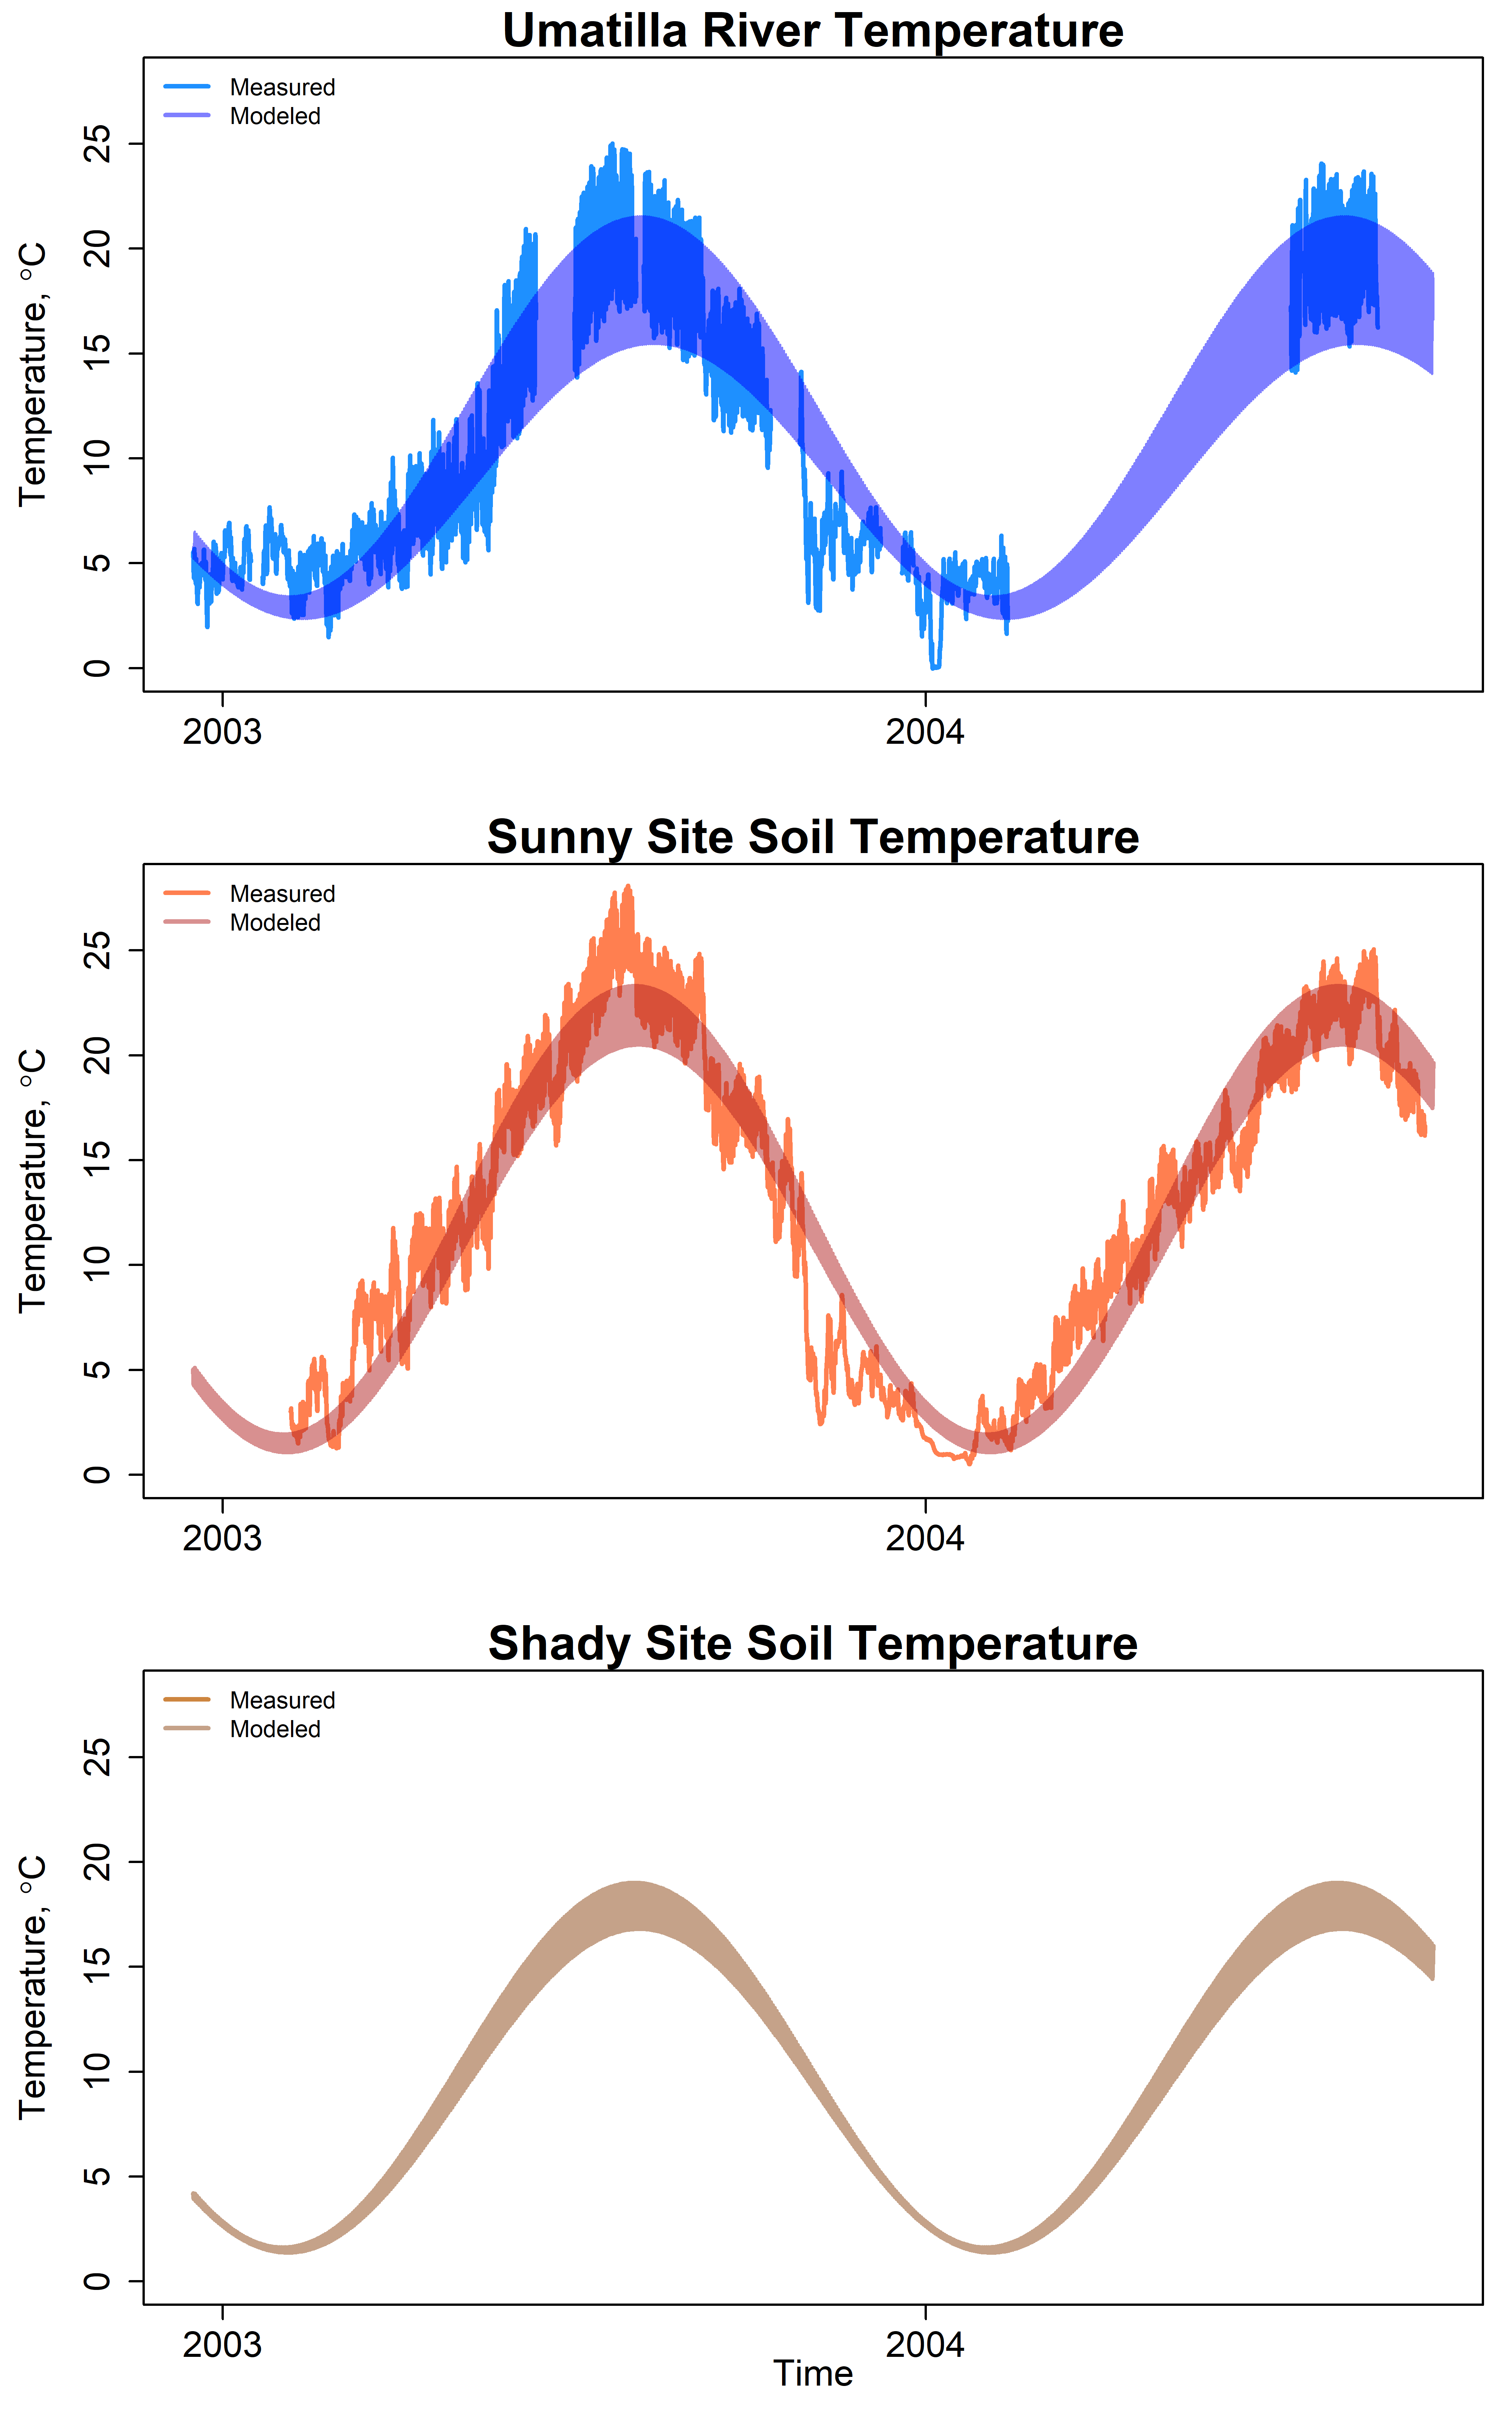
\includegraphics[width = 0.6\textwidth]{Figures/BoundaryInputs.png}
    \caption{Measured and modeled boundary inputs. River temperature was modeled using measured Umatilla River temperature (top). The sunny site soil temperature was modeled from a weather station located adjacent to the Umatilla river (middle). Shady temperature (bottom).}
    \label{fig:IskulpaaInputTemps}
\end{figure}



%\textbf{Hydraulic Conductivity (\textit{K})} & & \\
%    \hspace{6pt} x-direction & 0.001157407 & m s$^{-1}$\\
%    \hspace{6pt} y-direction & 0.0001157407 & m s$^{-1}$\\
%    \hspace{6pt} z-direction & 0.0001157407 & m s$^{-1}$\\ 
    



\section{Results}
%The amount of heat transferred through the unsaturated sediments of the floodplain is dependent upon the thickness of that unsaturated sediment layer.

Figure \ref{fig:dailyAnnualK100} shows temperature across flow path length for shaded (top) and sunny (bottom) model scenarios. The model shown had 1.0 meter of unsaturated floodplain sediment overlying the hyporheic zone and a hydraulic conductivity value of 100 m/day. At short flow path lengths, there was effectively no difference in temperature between shady and sunny floodplain scenarios (Figure \ref{fig:dailyAnnualK100}, left panel). The primary differences between the shaded and sunny floodplain model scenarios occurred at flow path lengths greater than ~200 meters. At these longer flow path lengths, the hyporheic zone temperature of the sunny floodplain was warmer across the entire year than the shaded floodplain (Figure \ref{fig:dailyAnnualK100}, right panel). The sunny floodplain scenario also leads to a wider temperature range of hyporheic temperature at longer flow paths.

Figure \ref{fig:dailyAnnualK400} shows results from the model scenario with a hydraulic conductivity value of 400 m/day (1.0 unsat. sediment thickness). The patterns shown explained in the paragraph above and shown in Figure \ref{fig:dailyAnnualK100} remain true for the model scenario with K = 400 m/day, except that the daily and annual temperature signals penetrate deeper into the aquifer (Note the y-axis scale change in the left panel from Figure \ref{fig:dailyAnnualK100} to Figure \ref{fig:dailyAnnualK400}).

\begin{figure}
    \centering
    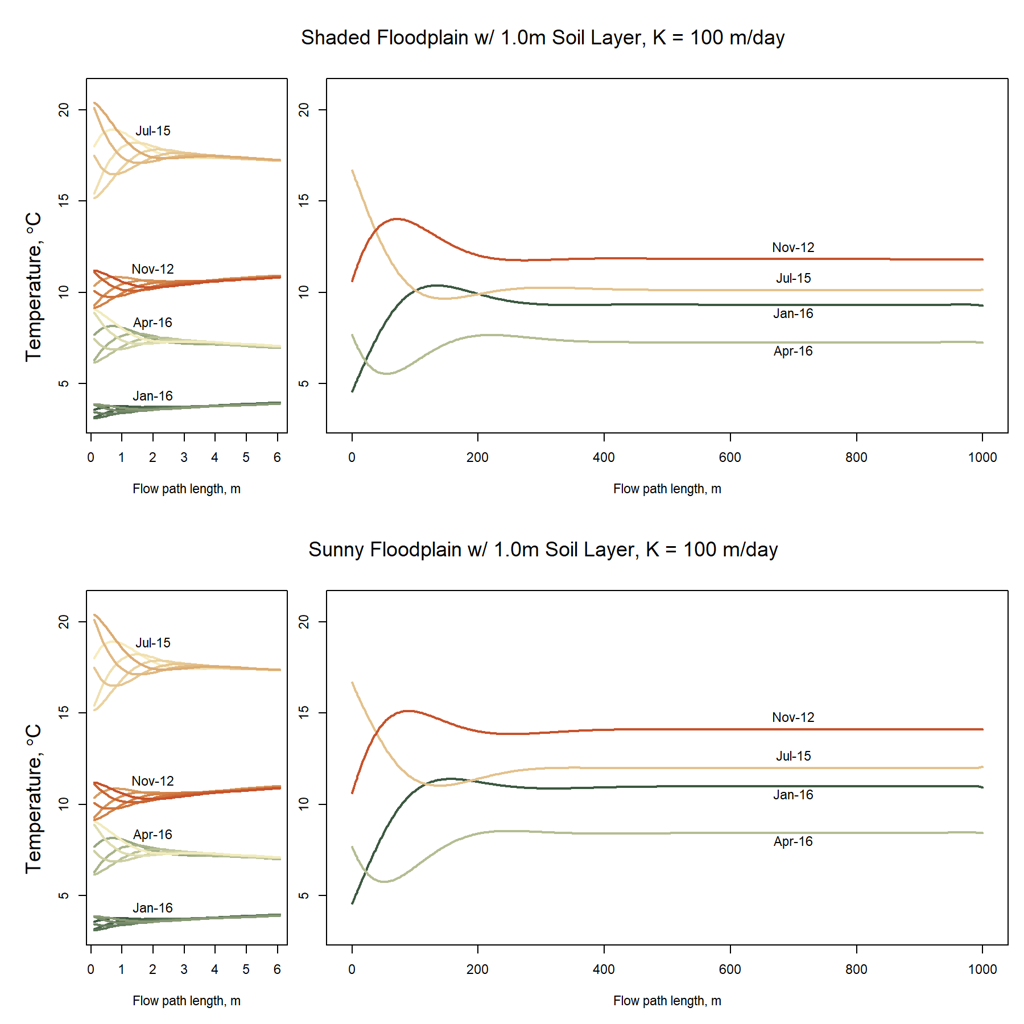
\includegraphics{Figures/shaded_and_sunny_1.0_daily_with_annual_k100.png}
    \caption{Simulated hyporheic zone temperatures from a shaded floodplain (top) and an unshaded floodplain (bottom). For Jan-16, Apr-16, Jul-15 and Nov 12, the left panel displays hyporheic temperatures at midnight, 4 AM, 8 AM, noon, 4 PM and 8 PM for each day, whereas the right panel displays the daily mean hyporheic zone temperatures. In the first few meters of the hyporheic zone, the daily signal is completely damped out (left). The annual signal (right) is not washed out until much deeper in the hyporheic zone. The model shown had a 1-meter thick unsaturated soil layer above the hyporheic zone and the hydraulic conductivity of the aquifer was 100 meters/day.}
    \label{fig:dailyAnnualK100}
\end{figure}

\begin{figure}
    \centering
    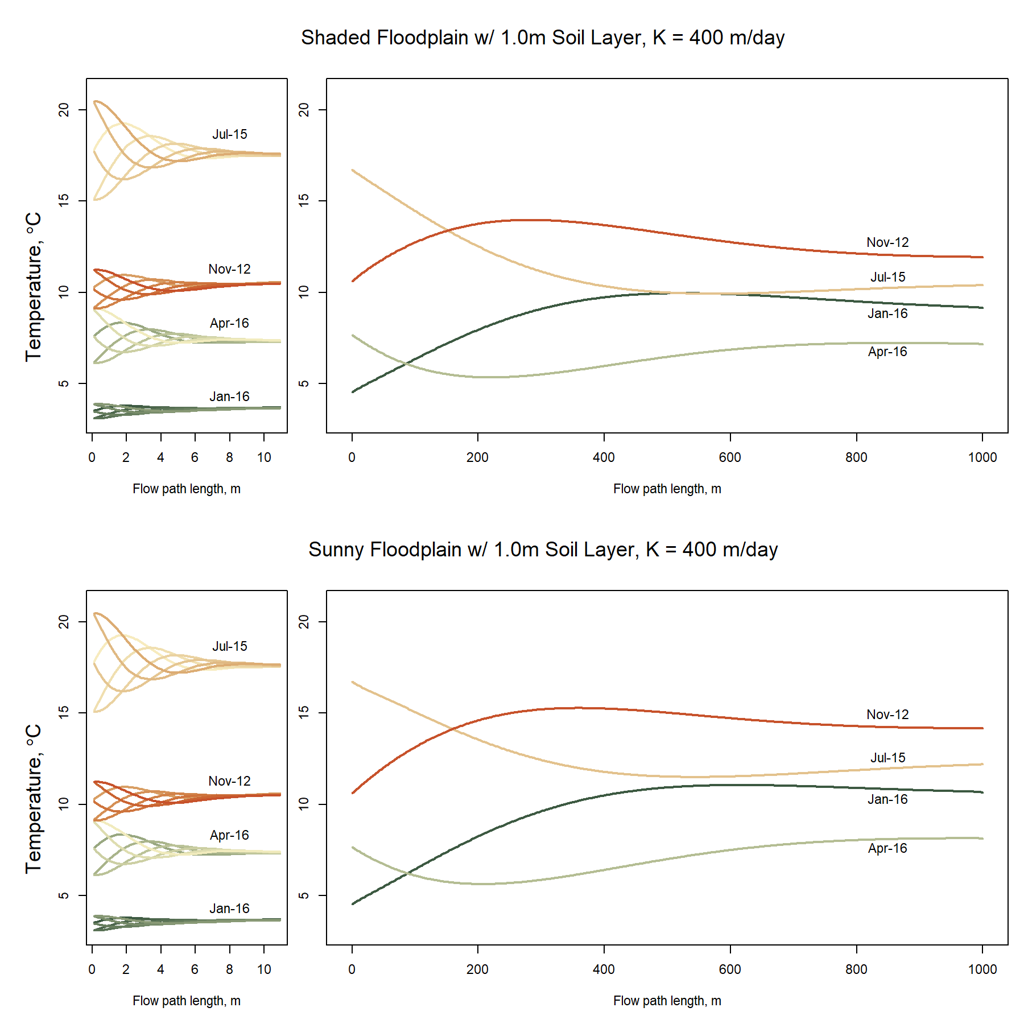
\includegraphics{Figures/shaded_and_sunny_1.0_daily_with_annual_k400.png}
    \caption{Simulated hyporheic zone temperatures from a shaded floodplain (top) and an unshaded floodplain (bottom). This model had an unsaturated soil layer of 1.0 meters thick and hydraulic conductivity of 400 meters/day. Note the change from Figure \ref{fig:dailyAnnualK100} of the x-axis scale of the left panel.}
    \label{fig:dailyAnnualK400}
\end{figure}

Model runs with higher hydraulic conductivity retain the river’s daily and annual signal much deeper into the hyporheic zone than the model runs with lower hydraulic conductivity (Figure \ref{fig:CompareK}). At very long flow paths, i.e. > 800 meters, the hyporheic temperature is similar across all modeled values of K. Because other model dimensions and parameters are kept the same, lower values of hydraulic conductivity result in slower hyporheic water travel times, thus the overlying floodplain temperature has more time to alter the temperature of this slower-moving water. 

\begin{figure}
    \centering
    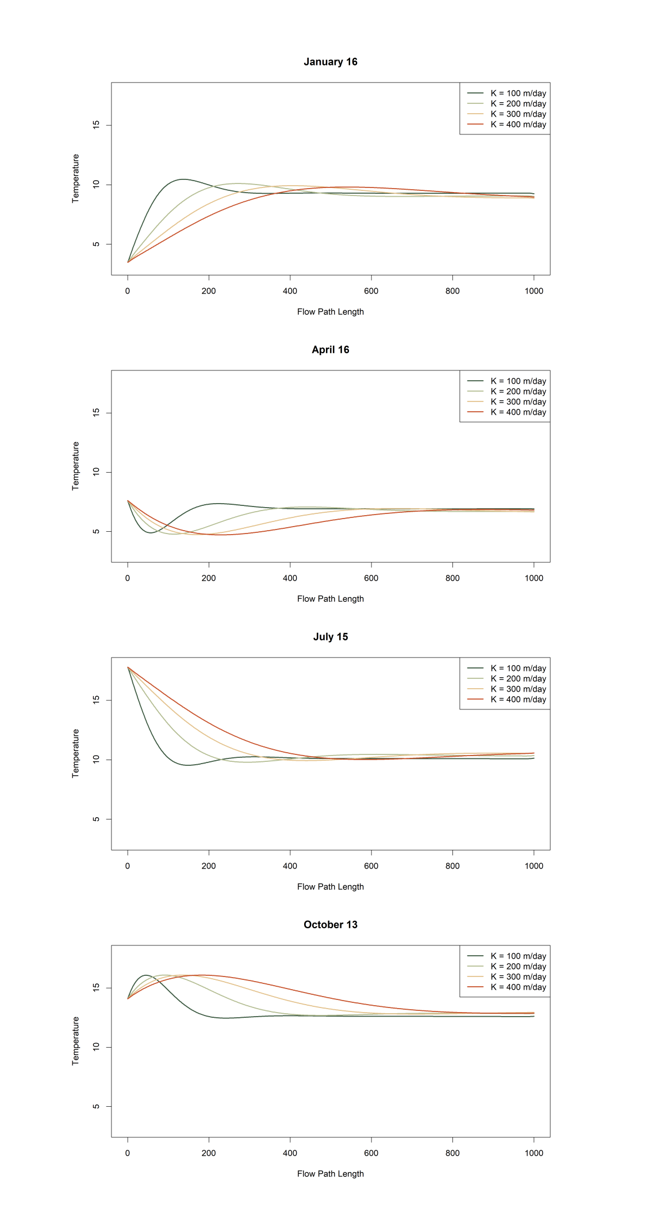
\includegraphics{Figures/Compare_K_Shady_1.0m.png}
    \caption{The effects on hyporheic temperatures of altering hydraulic conductivity, K, on a shaded floodplain with uniform soil layer thickness of 1.0 meters. As K increases, the river temperature sine wave flattens out and penetrates deeper into the aquifer, but all values of K come to the same temperature at very long flow paths >800 m.}
    \label{fig:CompareK}
\end{figure}


As the depth of the overlying floodplain soil increases, the effect of the temperature on the floodplain surface is diminished (Figures \ref{fig:thicknessK100}, \ref{fig:thicknessK400}). In shallow hyporheic zones, i.e. thin overlying soil layer, the surface temperature effects hyporheic water at shorter hyporheic flow path lengths. Whereas in deep hyporheic zones, i.e. thick overlying soil layer, the surface temperature does not have much of an effect until longer flow paths. Because most of the water upwelling form the hyporheic zone to the stream channel is from short flow paths \cite{Cardenas2008ResidenceExchange}, the degree to which a floodplain is shaded will have more of an effect on stream channel temperature where the overlying floodplain sediment is thin.

\begin{figure}
    \centering
    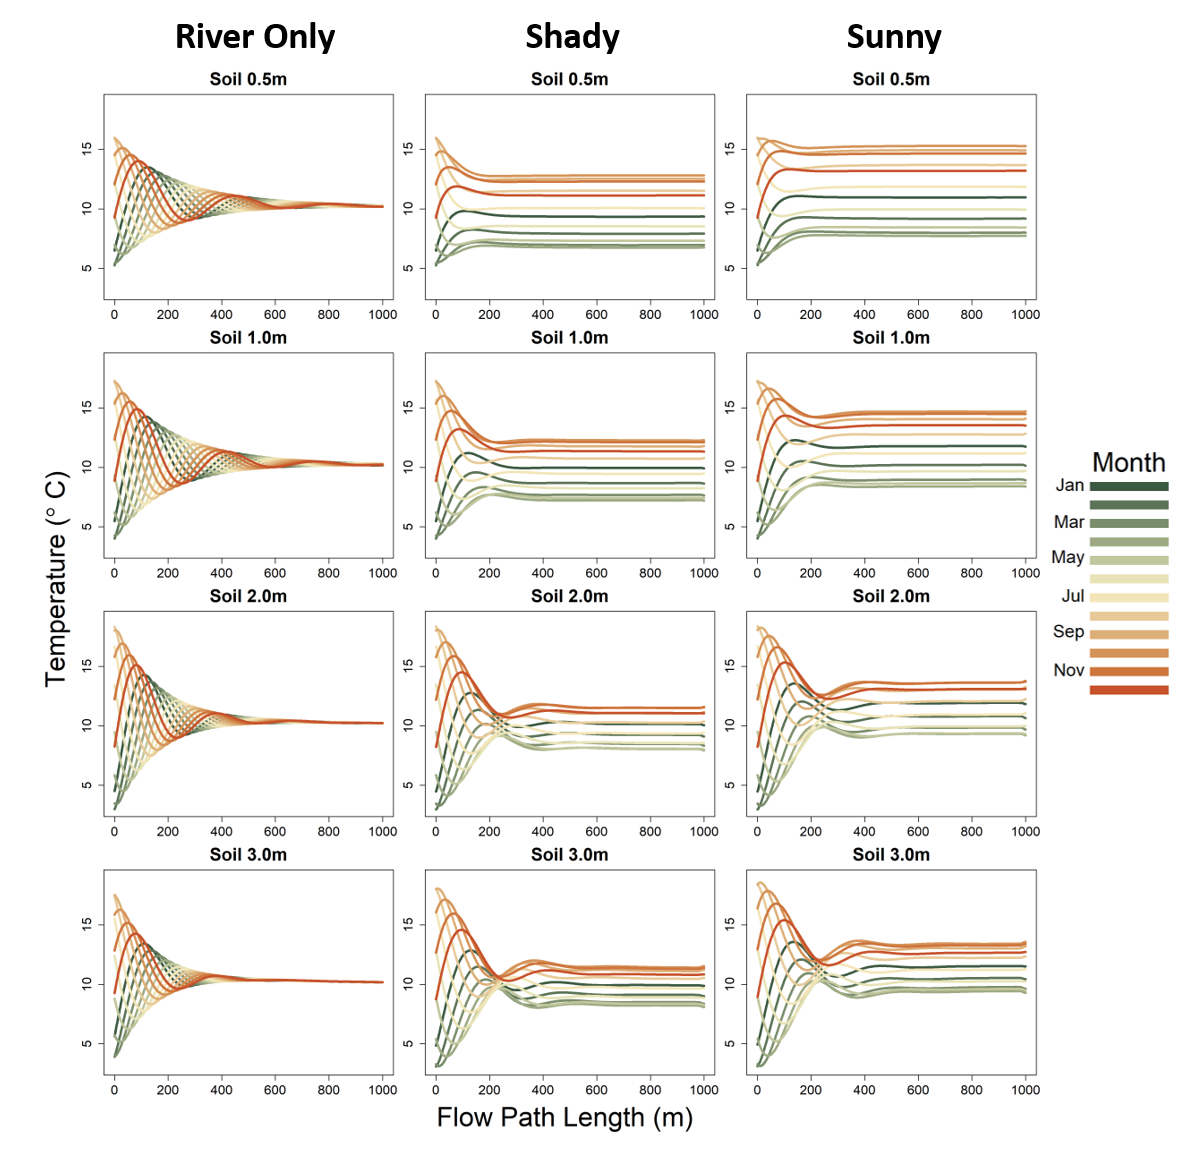
\includegraphics{Figures/compare_thickness_and_shade_k_100_w_riveronly_finalized.png}
    \caption{Hyporheic zone temperatures with increasing depth of overlying unsaturated soil, under different floodplain surface boundary conditions: no surface temperature (left), surface temperature reflective of a shaded floodplain (middle), and surface temperature reflective of a sunny floodplain (right). This model had a hydraulic conductivity, K, value of 100 meters/day.}
    \label{fig:thicknessK100}
\end{figure}

\begin{figure}
    \centering
    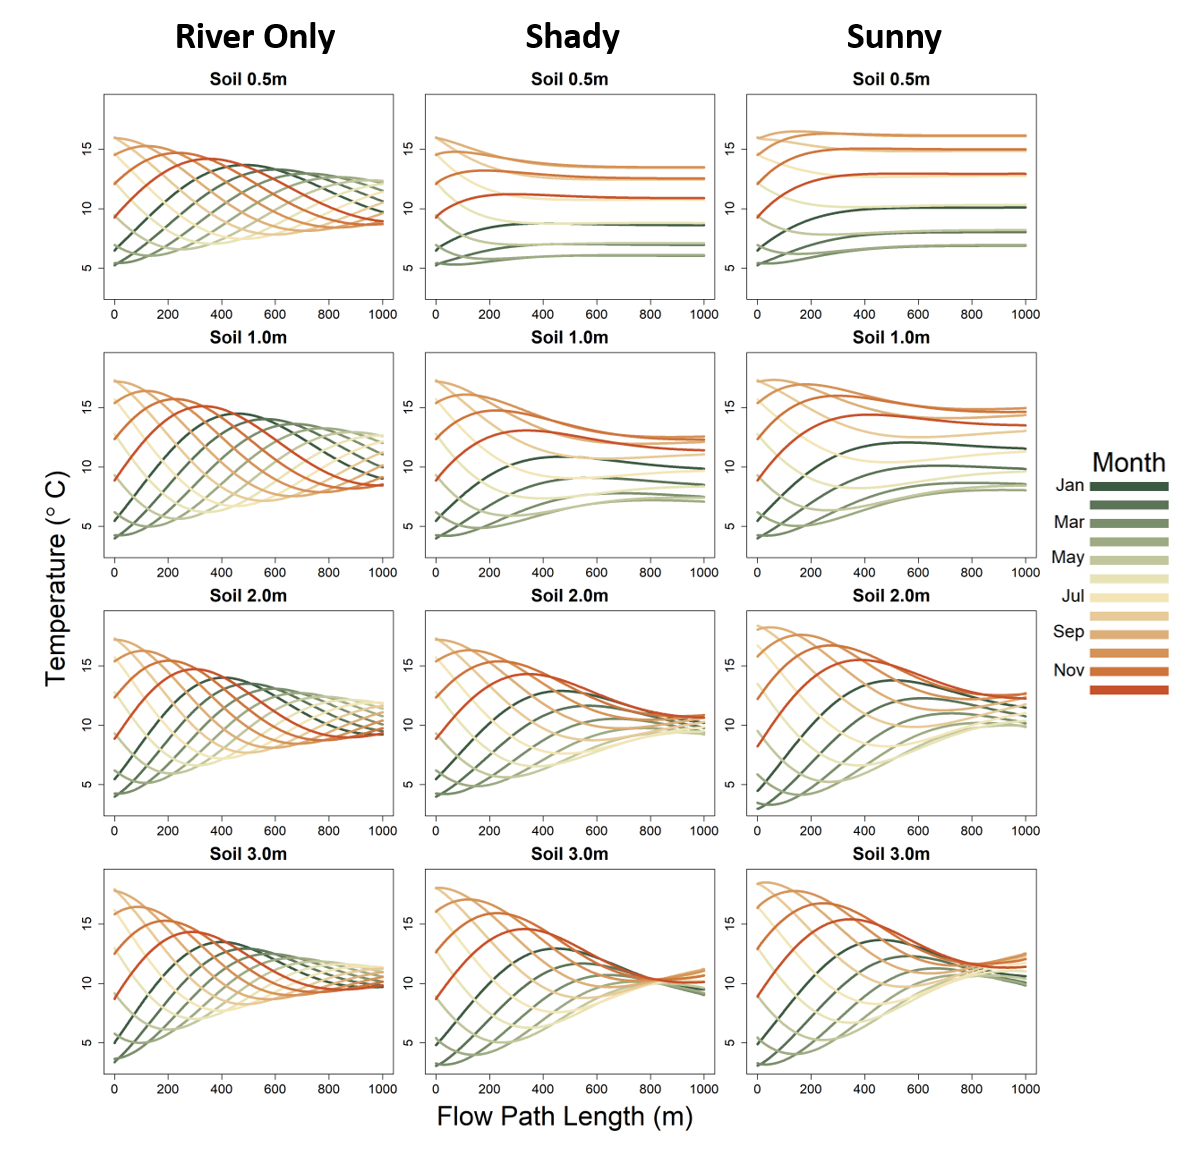
\includegraphics{Figures/compare_thickness_and_shade_k_400_w_riveronly_finalized.png}
    \caption{Hyporheic zone temperatures with increasing depth of overlying unsaturated soil, under different floodplain surface boundary conditions: no surface temperature (left), surface temperature reflective of a shaded floodplain (middle), and surface temperature reflective of a sunny floodplain (right). This model had a hydraulic conductivity, K, value of 400 meters/day.}
    \label{fig:thicknessK400}
\end{figure}

\end{document}
